% NeurIPS appendix: extended aleatoric analysis (moved from main text; nothing deleted)

\section{Extended aleatoric analysis}
\label{app:aleatoric_supp}

Material in this appendix supports §\ref{sec:aleatoric}: threshold sensitivity for copycat merging (evidence for a two-sentence conclusion in the main text), full Apelblat fit-quality diagnostics, and the planned cross-database check.

\subsection{Threshold sensitivity for copycat merging ($\theta_{B'}$)}
\label{app:threshold_sensitivity}

The threshold $\theta_{B'}$ controls a trade-off: too small a value
leaves obvious copies in the multi-source pool where they deflate
$\epsA$ artificially; too large a value merges genuinely agreeing labs,
shrinks the multi-source pool, and inflates $\epsA$ among the smaller
remaining pairs.  Figure~\ref{fig:threshold_sweep} shows the empirical
curve.  Below $\theta = 0.007$ very few additional unions are made: the
multi-source pair count barely decreases (from \numval{566} at $\theta
= 0$ to \numval{521} at $\theta = 0.007$, 8\,\% loss) and $\epsA$ rises
only 8\,\% (from \numval{0.091} to \numval{0.098}).  Between $\theta =
0.010$ and $\theta = 0.020$ there is a cliff in the pair count: from
\numval{484} pairs to \numval{378} pairs, a loss of \numval{106} pairs
over a 0.01-log-S interval (more than the entire loss for $\theta \in
[0, 0.01]$).  At the same time $\epsA$ jumps by 21\,\%, from
\numval{0.105} to \numval{0.127}.  Beyond $\theta = 0.05$ the
multi-source pool has more than halved.  We therefore adopt $\theta =
0.01$ as the conservative upper edge of the ``copycats-only'' region:
it merges the detectable copies while preserving the largest possible
multi-source pool for downstream analysis.

\begin{figure}[h]
  \centering
  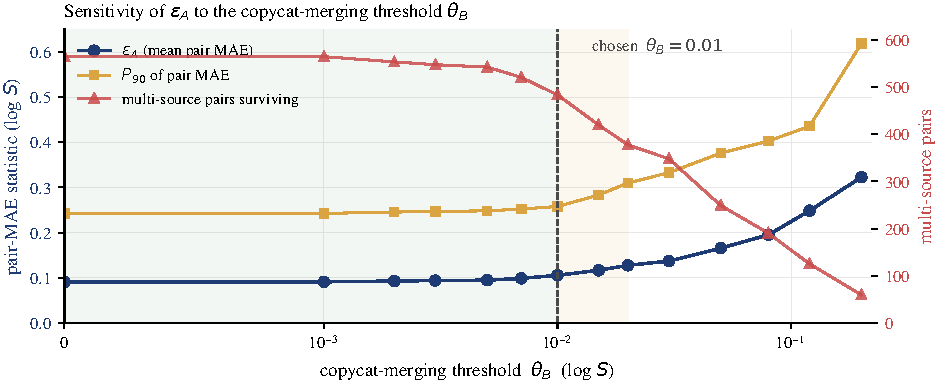
\includegraphics[width=0.9\linewidth]{figures/fig_threshold_sweep.pdf}
  \caption{Sensitivity of $\epsA$ and the multi-source pair count to the
    copycat-merging threshold $\theta_B$.  The chosen value $\theta_B =
    0.01$ (dashed line) sits at the upper edge of the shaded ``safe''
    region, where each merged pair is a genuine copy.  The shaded
    ``cliff'' region $[0.01, 0.02]$ loses $\numval{106}$ multi-source
    pairs --- more than the entire loss incurred between $0$ and
    $0.01$.}
  \label{fig:threshold_sweep}
\end{figure}

\subsection{Apelblat fit-quality diagnostics}
\label{app:apelblat_diagnostics}

Figure~\ref{fig:apelblat}(a) shows the fit-quality distribution: median
$R^2 = 0.9993$, \numval{99.3\,\%} of fits reach $R^2 \geq 0.95$,
\numval{94.9\,\%} reach $R^2 \geq 0.99$.  Thermodynamic monotonicity is
similarly strong: \numval{98.5\,\%} of triples are strictly
monotone-increasing in temperature and only \numval{1} triple shows a
single-step drop exceeding $1$~log~S.
Figure~\ref{fig:apelblat}(b) shows the distribution of per-fit
temperature coverage $\Delta T = T_{\max} - T_{\min}$.  The median
fit spans \numval{30}~K and only a small minority of fits cover less
than the 5~K minimum required for cross-group interpolation
(§\ref{sec:epsA}), confirming that the Apelblat framework supports
aleatoric analysis on the majority of the multi-source pool without
extrapolation.

\begin{figure}[h]
  \centering
  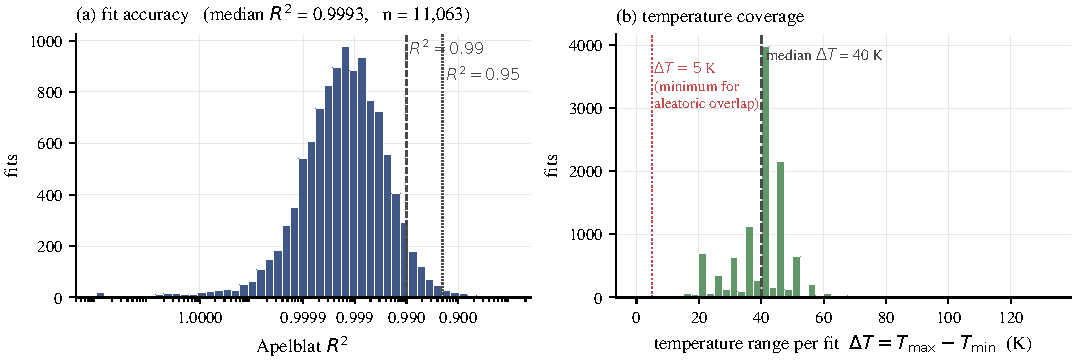
\includegraphics[width=\linewidth]{figures/fig_apelblat_quality.pdf}
  \caption{Apelblat fit quality.  \textbf{(a)}~$R^2$ distribution on a
    reversed log scale ($1 - R^2$ axis).  Most fits have
    $R^2 > 0.99$.  \textbf{(b)}~Temperature coverage $\Delta T$ per
    fit.  Most fits cover more than the 5~K minimum needed for aleatoric
    interpolation; the median fit spans \numval{30}~K.}
  \label{fig:apelblat}
\end{figure}
